\documentclass[12pt,tikz]{standalone}
\pdfinfoomitdate 1
\pdfsuppressptexinfo 1
\pdftrailerid{}
\usepackage[utf8]{inputenc}
\usepackage{amsmath}
\usepackage{pgfplots}
\usepackage{tikz}
\pagestyle{empty}
\definecolor{MyBlue}{RGB}{85,130,180}

\begin{document}
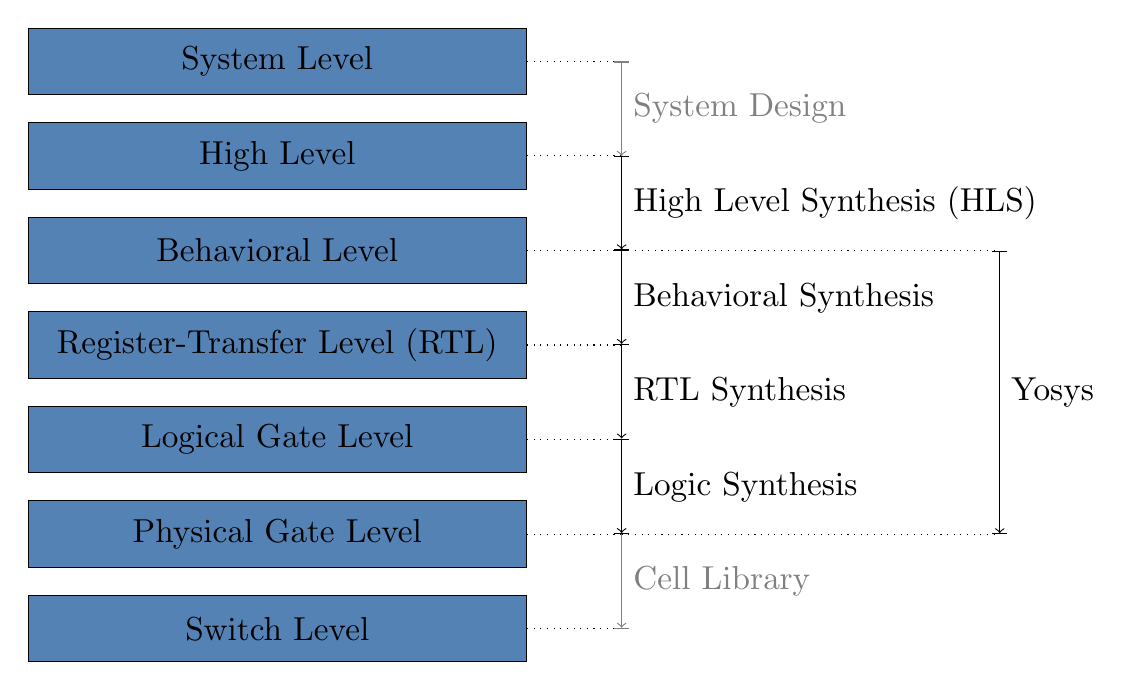
\begin{tikzpicture}[scale=1.2, every node/.style={transform shape}]
    \tikzstyle{lvl} = [draw, fill=MyBlue, rectangle, minimum height=2em, minimum width=15em]
    \node[lvl] (sys) {System Level};
    \node[lvl] (hl) [below of=sys] {High Level};
    \node[lvl] (beh) [below of=hl] {Behavioral Level};
    \node[lvl] (rtl) [below of=beh] {Register-Transfer Level (RTL)};
    \node[lvl] (lg) [below of=rtl] {Logical Gate Level};
    \node[lvl] (pg) [below of=lg] {Physical Gate Level};
    \node[lvl] (sw) [below of=pg] {Switch Level};

    \draw[dotted] (sys.east)  -- ++(1,0) coordinate (sysx);
    \draw[dotted] (hl.east)  -- ++(1,0) coordinate (hlx);
    \draw[dotted] (beh.east) -- ++(1,0) coordinate (behx);
    \draw[dotted] (rtl.east) -- ++(1,0) coordinate (rtlx);
    \draw[dotted] (lg.east)  -- ++(1,0) coordinate (lgx);
    \draw[dotted] (pg.east)  -- ++(1,0) coordinate (pgx);
    \draw[dotted] (sw.east)  -- ++(1,0) coordinate (swx);

    \draw[gray,|->] (sysx) -- node[right] {System Design} (hlx);
    \draw[|->|] (hlx) -- node[right] {High Level Synthesis (HLS)} (behx);
    \draw[->|] (behx) -- node[right] {Behavioral Synthesis} (rtlx);
    \draw[->|] (rtlx) -- node[right] {RTL Synthesis} (lgx);
    \draw[->|] (lgx) -- node[right] {Logic Synthesis} (pgx);
    \draw[gray,->|] (pgx) -- node[right] {Cell Library} (swx);

    \draw[dotted] (behx) -- ++(4,0) coordinate (a);
    \draw[dotted] (pgx) -- ++(4,0) coordinate (b);
    \draw[|->|] (a) -- node[right] {Yosys} (b);
\end{tikzpicture}
\end{document}
